\section{Laboratory work implementation}

\subsection{Tasks and Points}

\begin{enumerate}
\item Realizarea unui joc
\item Folosirea unei librării cross platform pentru a realiza o aplicație platform (aplicația poate fi compilată atât pe Android cât și iOS)
\end{enumerate}

\subsection{Analiza lucrarii de laborator}

\begin{enumerate}
\item Primul pas a fost inițializarea unui nou repozitoriu pe GitHub și clonarea acestuia pe calculatorul personal: \url{https://github.com/emirovschi/MIDPS\-4}.
\item Proiectul a fost creat utilizând Projeny\cite{Projeny}. Acesta oferă posibilitatea de a organiza codul în module care pot fi configurate individual pentru diferite platforme.
\item Projeny genereaza proiect de tip Unity3D\cite{Unity3D}. Avantajele acestui instrument este posibilitatea de a crea ușor jocuri pentru mai multe platforme, este costumizabil, extensibil și ușor de utilizat.

\begin{minipage}{\linewidth}
	\centering
	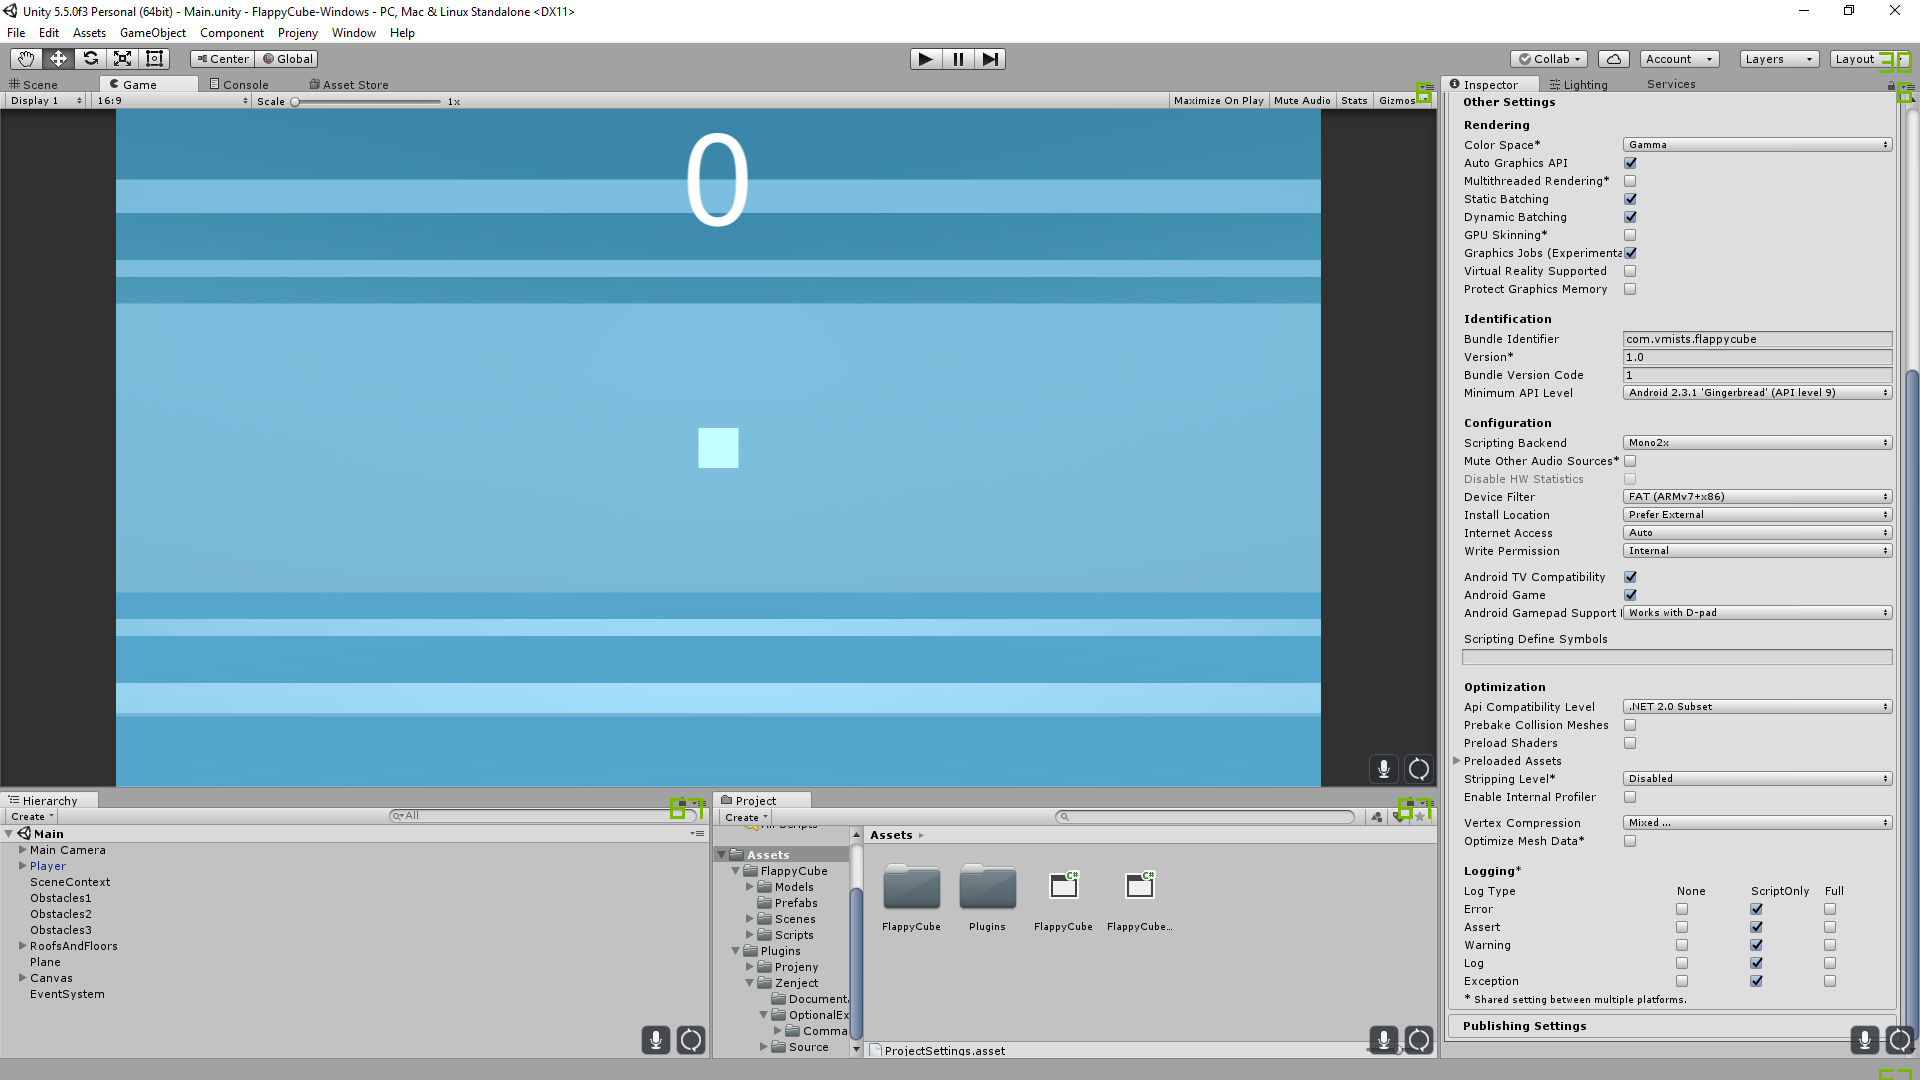
\includegraphics[width=17cm]{unity}
	\captionof{figure}{Interfața Unity3D}
\end{minipage}
\break

\item Unity3D utilizeaza platforma .NET respectiv limbajul de programare este C\#\cite{CSharp}. Astfel pentru redactarea codului am folosit Visual Studio\cite{vs}.
\item La elaborarea acestui proiect am folosit biblioteca Zenject\cite{Zenject}. Ea conține un sistem de Inversion Of Control similar cu cel din Spring pentru Java. Aici regulele de injectre a dependențelor sunt definite cu ajutorul unor comenzi specifice. Un alt avantaj al acestei biblioteci este compatibilitatea sa cu Unity3D oferind posibilitatea de a inject dependențe in componentele controlate de engine.

\begin{minipage}{\linewidth}
	\centering
	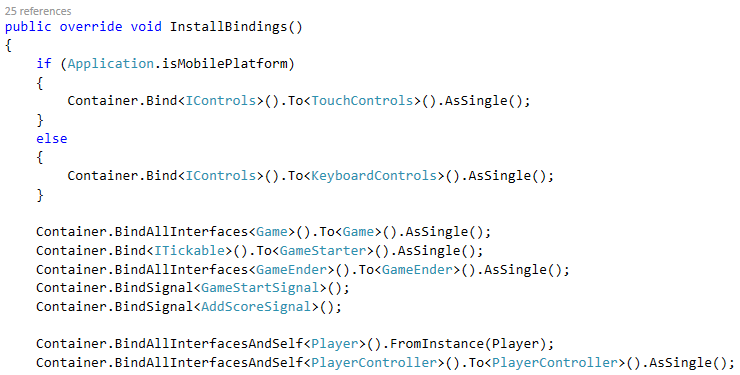
\includegraphics[width=17cm]{zenject}
	\captionof{figure}{Exemplu de configurare a dependențelor in Zenject}
\end{minipage}
\break

\item Pentru simplicitatea am folosit modele 3D primitive existente deja în Unity3D, partea personalizată fiind reprezentată de componentele implementate in C\#.
\item Un element important al jocului dat este generarea procedurală a lumii. Aceasta are loc prin generarea unei liste de obstacle și repoziționarea lor când sunt 

\end{enumerate}

\break
\subsection{Imagini}

\begin{figure}[ht]
	\centering
	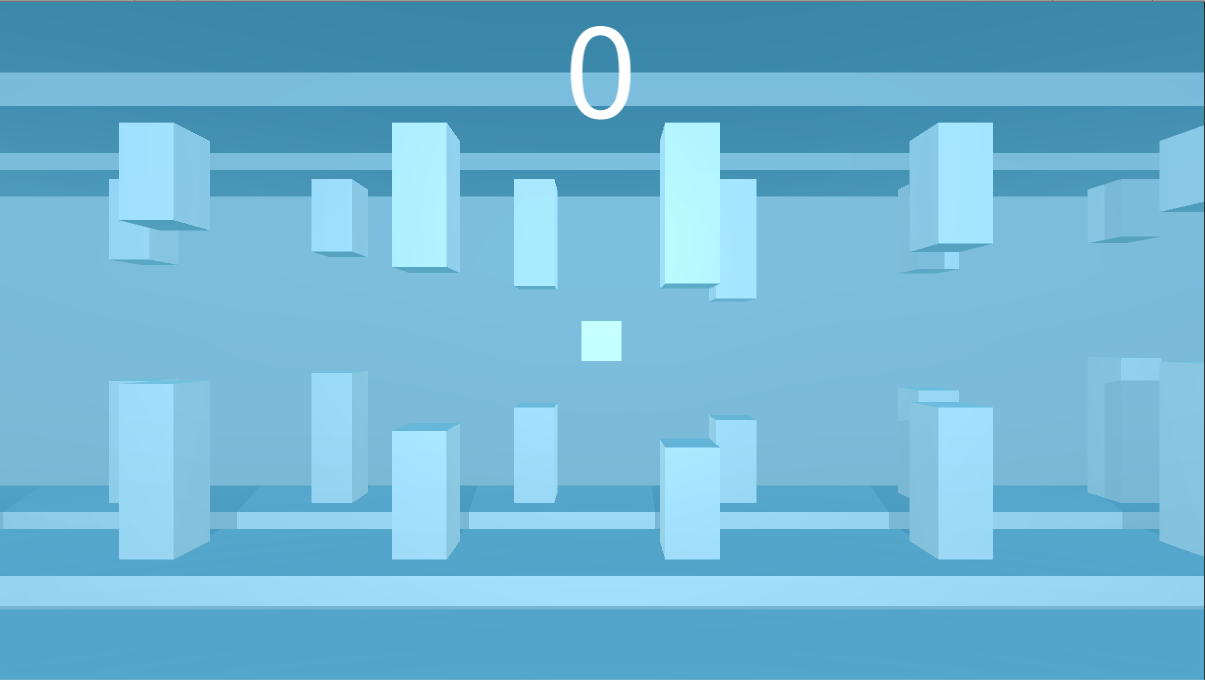
\includegraphics[width=9.7cm]{start}
	\caption{Scene inițială}
\end{figure}

\begin{figure}[ht]
	\centering
	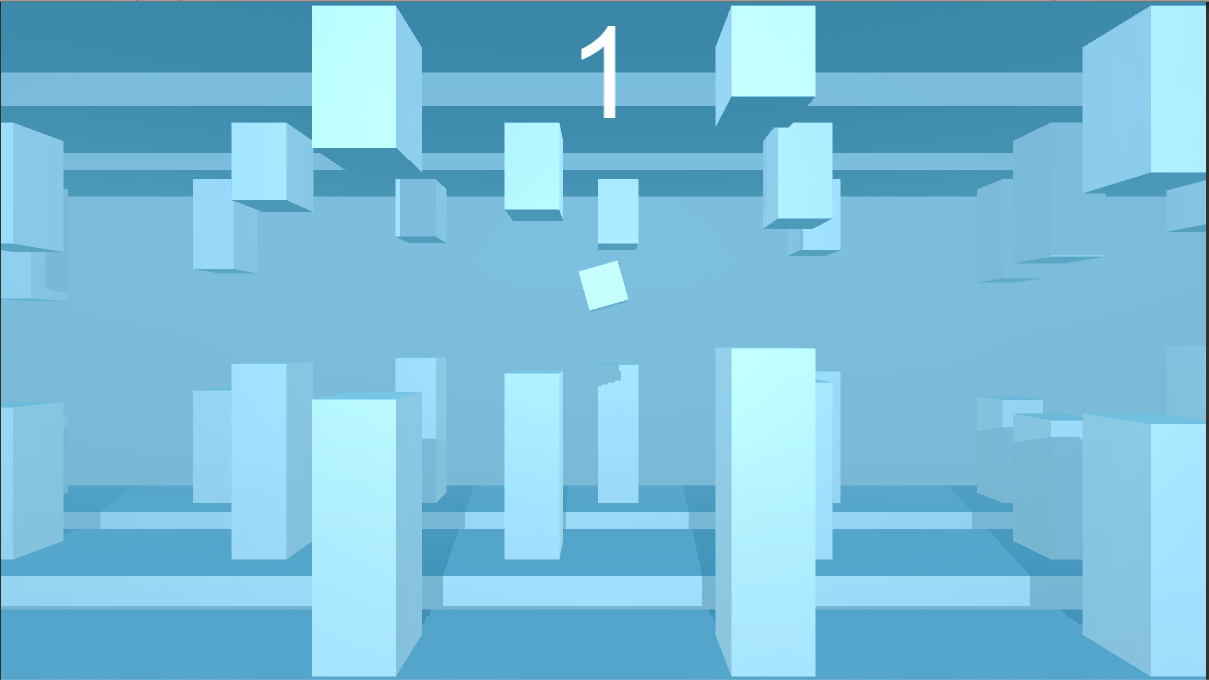
\includegraphics[width=9.7cm]{obstacles}
	\caption{Exemplu de lume generată procedural}
\end{figure}

\begin{figure}[ht]
	\centering
	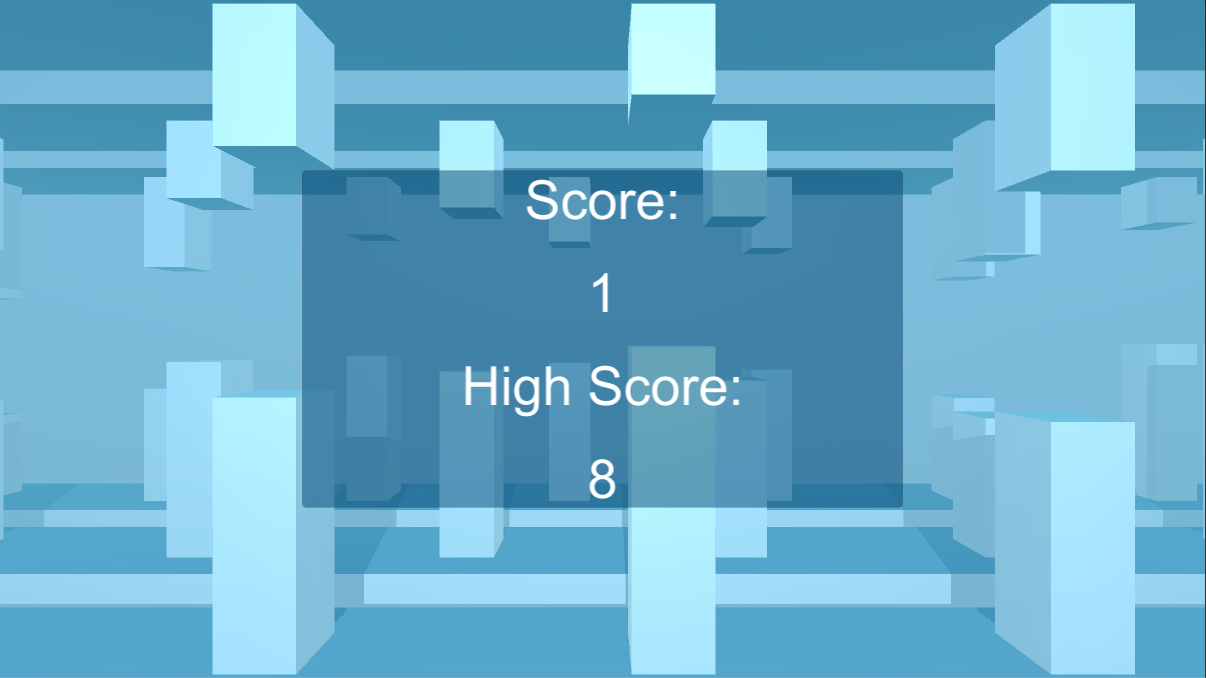
\includegraphics[width=9.7cm]{end}
	\caption{Scene de finisare și afișarea a scorului final}
\end{figure}

\clearpage